\documentclass[10pt,a4paper]{article}
\usepackage{amsmath}
\usepackage{amssymb}
\usepackage{graphicx}
\usepackage{color}
\usepackage{fancyhdr}
\usepackage{fancyvrb}
\usepackage[margin=3.5cm]{geometry}
\usepackage{framed}
\usepackage{enumerate}
\usepackage{textcomp}
\usepackage{float}
\def\ket#1{\left|#1\right\rangle}
\def\bra#1{\left\langle#1\right|}
\def\braket#1{\left\langle#1\right\rangle}

\definecolor{linkcol}{rgb}{0.0, 0.0, 0.7}
\usepackage[colorlinks=true,urlcolor=linkcol,citecolor=black,linkcolor=linkcol]{hyperref}

\setcounter{section}{10}
\renewcommand\thesection{\arabic{section}}
\renewcommand\thesubsection{\thesection.\arabic{subsection}}

\fancyhf{}
\lhead{\tiny Y.~D.~Chong (2020)}
\rhead{\scriptsize MH2801: Complex Methods for the Sciences}
\lfoot{}
\rfoot{\thepage}
\pagestyle{fancy}

\begin{document}

\setcounter{page}{94}

\section{Solutions for Selected Problems}

\subsection*{0. Mathematical Functions}

\begin{enumerate}
\item[2.]
To prove that $\exp(x+y) = \exp(x)\,\exp(y)$, we employ the infinite
series formula \begin{equation}
  \exp(x) = \sum_{n=0}^\infty\frac{x^n}{n!}.
\end{equation}
Here, for notational convenience, we let the sum start from $n = 0$,
so that the leading term $1$ in the definition of the exponential is
grouped with the rest of the sum as its first term. This relies on the
understanding that $0! \equiv 1$, and that $x^0 = 1$ (the latter is
consistent with the generalized definition of the power operation; but
to avoid circular logic, treat this as the \emph{definition} of $x^0$
just for the sake of this proof). We begin by substituting the series
formula into the right-hand side of our target equation:
\begin{equation}
  \exp(x)\exp(x) = \left(\sum_{n=0}^\infty\frac{x^n}{n!}\right)\;\left(\sum_{m=0}^\infty\frac{y^m}{m!}\right).
\end{equation}
Note that we use the symbol $n$ for the first sum, and the symbol
$m$ for the second sum; $n$ and $m$ are bound variables, whose
terms run over the values specified by the summation signs. The actual
choice of symbol used in either sum is unimportant, except that \emph{we
must not use the same symbol for both sums}, because the two variables
belong to distinct sums. In other words:
\begin{equation*}
  \exp(x)\exp(x) \ne \left(\sum_{n=0}^\infty\frac{x^n}{n!}\right)\;\left(\sum_{n=0}^\infty\frac{y^n}{n!}\right). \quad(\text{Nonsense expression!})
\end{equation*}
Next, we make use of the fact that the product of two series can be
written as a double sum:
\begin{equation}
  \exp(x)\exp(x) = \sum_{n=0}^\infty \sum_{m=0}^\infty \frac{x^n}{n!} \frac{y^m}{m!}.
\end{equation}
Here, we are summing over all possible pair-wise combinations of $n$
and $m$, which is precisely what happens when one expands the product
of two series according to the usual rules of algebra. The next step
is to perform a \emph{change of variables} on $m$ and $n$. In the
above expression, we are summing over all non-negative integer $m$ and
$n$; however, the bound variable $n$ can be re-expressed in terms of a
newly-defined variable,
\begin{equation}
  N = m + n.
\end{equation}
In the original double sum, $n$ and $m$ both run from $0$ to
$+\infty$, so it follows that their sum $N$ runs from $0$ to
$+\infty$. For each given value of $N$, we can write $n = N - m$, and
moreover the allowed values of $m$ would only go from $0$ to $N$ (it
can't exceed $N$, otherwise $n$ would be negative). In this way, the
double sum is converted to
\begin{equation}
  \exp(x)\exp(x) = \sum_{N=0}^\infty \sum_{m=0}^N \frac{x^{N-m}}{(N-m)!} \frac{y^m}{m!}
\end{equation}
Note that after this change of variables, the two summation signs are
no longer interchangeable. In the $\sum_{m=0}^N$ sign, the variable
$N$ appears in the upper limit, so this needs to be written to the
right of $\sum_{N=0}^\infty$. One sum is thus ``encapsulated'' inside
the other; we could write the algebraic expression more rigorously
like this:
\begin{equation}
  \exp(x)\exp(x) = \sum_{N=0}^\infty \left(\sum_{m=0}^N \frac{x^{N-m}}{(N-m)!} \frac{y^m}{m!}\right).
\end{equation}
Finally, we use the binomial theorem to simplify the inner sum:
\begin{equation}
  \exp(x)\exp(x) = \sum_{N=0}^\infty \frac{\left(x + y\right)^N}{N!}, \;\;\;\text{since} \;\; (x+y)^N = \sum_{m=0}^N \frac{N!}{m!(N-m)!} x^{N-m} \, y^m.
\end{equation}
Referring again to the series definition of the exponential, we obtain
the desired result:
\begin{equation}
  \exp(x)\exp(x) = \exp(x+y)
\end{equation}

\item[4.]
The definition of non-natural powers is
\begin{equation}
  a^b = \exp[b\ln(a)].
\end{equation}
Let $a = \exp(1) = e$ and $b = x$. Then
\begin{equation}
  [\exp(1)]^x = \exp\left[x\ln\Big(\exp(1)\Big)\right].
\end{equation}
Since the logarithm is the inverse of the exponential function,
$\ln(\exp(1)) = 1$. Hence,
\begin{equation}
  e^x = \exp(x).
\end{equation}
\end{enumerate}

\subsection*{1. Derivatives}

\begin{enumerate}
\item[2.]
If $y = \ln(x)$, it follows from the definition of the logarithm that
\begin{equation}
  \exp(y) = x.
\end{equation}
Taking $d/dx$ on both sides, and using the product rule, gives
\begin{equation}
  \frac{dy}{dx} \, \exp(y) = 1 \;\;\; \Rightarrow \frac{dy}{dx} = \frac{1}{\exp(y)} = \frac{1}{x}.
\end{equation}

\item[8.]
For an ordinary differential equation for a scalar (one-component)
function of order $n$, the general solution must contain $n$
independent variables. In this case, $\vec{v}$ is a two-component
function, so it requires $2n$ indpendent variables. The differential
equation
\begin{equation}
  \frac{d\vec{v}}{dx} = \mathbf{A} \vec{v}
\end{equation}
has order $n = 1$, so a total of 2 independent variables is required
for the general solution.

Let $u$ be an eigenvector of $\mathbf{A}$ with eigenvalue $\lambda$,
and suppose that $\vec{v}(x) = \vec{u}\,e^{\lambda x}$ (note that
$\vec{u}$ itself does not depend on $x$). Then
\begin{align}
  \frac{d\vec{v}}{dx} &= \vec{u} \frac{d}{dx}\left(e^{\lambda x}\right) \\
  &= \lambda \, \vec{u}\, e^{\lambda x} \\
  &= \left(\mathbf{A} \vec{u}\right) e^{\lambda x} \\
  &= \mathbf{A} \left(\vec{u} e^{\lambda x}\right) \\
  &= \mathbf{A} \vec{v}(x).
\end{align}
Hence, $\vec{v}(x)$ satisfies the desired differential equation.

Let $\vec{u}_1$ and $\vec{u}_2$ be the eigenvectors of $\mathbf{A}$,
with eigenvalues $\lambda_1$ and $\lambda_2$. The general solutions
will be
\begin{equation}
  \vec{v}(x) = c_1 \vec{u}_1 e^{\lambda_1 x} + c_2 \vec{u}_2 e^{\lambda_2 x},
\end{equation}
where $c_1$ and $c_2$ are independent variables.
\end{enumerate}

\subsection*{2. Integrals}

\begin{enumerate}
\item[4.]
Let us define
\begin{equation}
  I(\gamma) = \int_0^1 \frac{x^\gamma - 1}{\ln(x)},
\end{equation}
so that $I(2)$ is our desired integral. To take the derivative, first
note that
\begin{equation}
  \frac{d}{d\gamma}(x^\gamma) = \ln(x)\,
  x^\gamma,
\end{equation}
which can be proven using the generalized definition of the power
operation. Thus,
\begin{align}
  \frac{d}{d\gamma} I(\gamma) &= \int_0^1 \frac{\ln(x) x^\gamma}{\ln(x)} \\
  &= \int_0^1 x^\gamma \\
  &= \frac{1}{1+\gamma}.
\end{align}
This can be integrated straightforwardly:
\begin{equation}
  I(\gamma) = \int \frac{d\gamma}{1+\gamma} = \ln(1+\gamma) + c,
\end{equation}
where $c$ is a constant of integration, which we now have to
determine.  Referring to the original definition of $I(\gamma)$,
observe that $I(0) = \int_0^1 (1 - 1)/\ln(x) = 0$. This implies that
$c = 0$.  Therefore, the answer is
\begin{equation}
  I(2) = \ln(3).
\end{equation}

\item[6.]
We are provided with the following ansatz for the solution to the
differential equation:
\begin{equation}
  y(t) = y(0) + \int_0^t dt' e^{-\gamma(t-t')} g(t').
\end{equation}
First, note that when $t = 0$, the integral's range shrinks to zero,
so the result is $y(0)$, as expected. In order to determine the
appropriate function $g$, we perform a derivative in $t$. The tricky
part is that $t$ appears in two places: in the upper range of the
integral, as well as in the integrand. So when we take the derivative,
there should be two distinct terms (see problem 5):
\begin{align}
  \frac{dy}{dt} &= \left[e^{-\gamma(t-t')} g(t')\right]_{t'=t} + \int_0^t dt'(-\gamma) \, e^{-\gamma(t-t')} \, g(t')\\
  &= g(t) - \gamma [y(t) - y(0)].
\end{align}
In the last step, we again made use of the ansatz for $y(t)$. Finally,
comparing this with the original differential equation for $y(t)$, we
find that
\begin{equation}
  g(t) - \gamma [y(t) - y(0)] = -\gamma y(t) + f(t) \;\;\; \Rightarrow \;\;\; g(t) = f(t) - \gamma y(0).
\end{equation}
Hence, the solution to the differential equation is
\begin{align}
  y(t) &= y(0) + \int_0^t dt' \, e^{-\gamma(t-t')} \,[f(t') - \gamma y(0)] \\
  &= y(0)\,e^{-\gamma t} + \int_0^t dt' \, e^{-\gamma(t-t')} f(t').
\end{align}
\end{enumerate}

\subsection*{3. Complex Numbers}

\begin{enumerate}
\item[2.]
Using the polar representation: let $z_1 = r_1 \exp(i\theta_1)$ and
$z_2 = r_2 \exp(i\theta_2)$. Then
\begin{align}
  \big|z_1\, z_2\big| &= \left|r_1 e^{i\theta_1} \, r_2 e^{i\theta_2}\right| \\
  &= \left|(r_1r_2)\,e^{i(\theta_1+\theta_2)}\right| \\
  &= r_1 r_2 \\
  &= |z_1|\, |z_2|.
\end{align}
Using the Cartesian representation: let $z_1 = x_1+iy_1$ and $z_2 =
x_2+iy_2$. For convenience, we evaluate the squared magnitude:
\begin{align}
  \big|z_1\, z_2\big|^2 &= \left|(x_1x_2 - y_1y_2) + i (x_1y_2+x_2y_1)\right|^2 \\
  &= (x_1x_2 - y_1y_2)^2 + (x_1y_2+x_2y_1)^2 \\
  &= x_1^2x_2^2 + y_1^2 y_2^2 + x_1^2y_2^2 + x_2^2 y_1^2 \\
  &= \left(x_1^2 + y_1^2\right)\left(x_2^2 + y_2^2\right) \\
  &= |z_1|^2 \, |z_2|^2.
\end{align}

\item[3.] Using the polar representation: let $z_1 = r_1
  \exp(i\theta_1)$ and $z_2 = r_2 \exp(i\theta_2)$. Then
\begin{align}\big(z_1\, z_2\big)^* &= \left(\left(r_1r_2\right) e^{i(\theta_1+\theta_2)}\right)^* \\ &= \left(r_1r_2\right) e^{-i(\theta_1+\theta_2)} \\
  &= \left(r_1 e^{-i\theta_1}\right) \left(r_2 e^{-i\theta_2}\right) \\
  &= z_1^* \, z_2^*.
\end{align}
Using the Cartesian representation: let $z_1 = x_1+iy_1$ and
$z_2 = x_2+iy_2$.
\begin{align}\big(z_1\, z_2\big)^* &= \left[\left(x_1x_2 - y_1y_2\right) + i \left(x_1y_2+x_2y_1\right)\right]^* \\
  &= \left(x_1x_2 - y_1y_2\right) - i \left(x_1y_2+x_2y_1\right) \\
  &= \left(x_1 - iy_1\right) \left(x_2 - iy_y\right) \\
  &= z_1^* \, z_2^*.
\end{align}

\item[4.]
The problem arises in this part of the chain: $i\cdot i =
\sqrt{-1}\,\sqrt{-1} = \sqrt{(-1)(-1)}$. The square root is a
non-integer power, and non-integer powers are not allowed to take part
in standard complex algebra equations in the same way as addition,
subtraction, multiplication, division, and integer powers.

As discussed in Chapter 7, square roots and other non-integer powers
have multiple values. The definition of the imaginary unit is often
written as $i = \sqrt{-1}$, but this is misleading. Actually,
$\sqrt{-1}$ has two legitimate values; one of these values is (by
definition) $i$, while the other value is $-i$.
\end{enumerate}

\subsection*{4. Complex Oscillations}

\begin{enumerate}
\item[4.]
The general solution is
\begin{equation}
  z(t) = A \exp\left[-i(\omega_1 - i \gamma) t\right].
\end{equation}
It can be verified by direct substitution that this is a solution to
the differential equation. It contains one free parameter, and the
differential equation is first-order, so it must be a general
solution.  Next,
\begin{align}
  \frac{d^2z}{dt^2} + 2 \gamma \frac{dz}{dt} &= (-i)^2(\omega_1 - i\gamma)^2 z(t) - 2i \gamma (\omega_1 - i \gamma) z(t) \\
  &= \left[- \omega_1^2 + \gamma^2 + 2i\gamma\omega_1 - 2i \gamma \omega_1 - 2\gamma^2)\right] z(t) \\
  &= -\left(\omega_1^2 + \gamma^2\right)z(t).
\end{align}
Hence, $z(t)$ obeys a damped harmonic oscillator equation with
$\omega_0^2 = \omega_1^2 + \gamma^2.$ This expression for the natural
frequency ensures that $\omega_0^2 > \gamma^2$ (assuming the
parameters $\gamma$ and $\omega_1$ are both real); hence, the
harmonic oscillator is always under-damped.
\end{enumerate}

\subsection*{5. Complex Waves}

\begin{enumerate}
\item[2.]
Writing $n = n' + i n''$, where $n'$ and $n''$ are real, the
travelling wave solutions are
\begin{equation}
  \psi(x) = A \exp\left[\pm i (n'+in'')\frac{\omega}{c} x\right].
\end{equation}
The magnitude and argument are:
\begin{align}
  \big|\psi(x)\big| &= |A| \exp\left[\mp n'' \frac{\omega}{c} x \right] \\
  \mathrm{arg}\big[\psi(x)\big] &= \mathrm{arg}(A) \pm n' \frac{\omega}{c} x.
\end{align}
The wave's propagation direction is determined by the argument: if the
argument increases with $x$ then it is right-moving, and if the
argument decreases with $x$ it is left-moving. Moreover, the wave is
said to experience amplification if its amplitude grows along the
propagation direction, and damping if its amplitude decreases along the
propagation direction.

Consider the upper choice of sign (i.e., $+$ for the $\pm$ symbol
and $-$ for the $\mp$ symbol). From the magnitude, we see that the
wave's amplitude decreases with $x$ if $n'' > 0$, and increases with
$x$ if $n'' < 0$. From the argument, the wave is right-moving if
$n' >0$, and left-moving if $n' < 0$. Hence, the wave is damped if
$n' n'' >0$ and amplified if $n' n'' < 0$.

(For example, consider the case $n' < 0$ and $n'' < 0$. The
amplitude increases with $x$ but the wave is moving in the $-x$
direction; this means the amplitude grows in the direction opposite to
the propagation direction, so the wave is damped.)

For the lower choice of sign, we see from the magnitdue that the
amplitude increases with $x$ if $n'' > 0$, and decreases with $x$
if $n'' < 0$. From the argument, we see that the wave is left-moving
if $n' >0$ and right-moving if $n' < 0$. Hence, the wave is damped
if $n' n'' >0$ and amplified if $n' n'' < 0$, exactly the same as in
the previous case.

Hence, whether the wave is amplified or damped only depends on the
relative signs of $n'$ and $n''$, and is independent of the
direction of propagation.
\end{enumerate}

\subsection*{6. Complex Derivatives}

\begin{enumerate}
\item[3.]
We will use the Cauchy-Riemann equations. Decompose $z$, $f$, and
$g$ into real and imaginary parts as follows: $z = x + i y$,
$f = u + i v$, and $g = p + i q$. Since $f(z)$ and $g(z)$ are
analytic in $D$, they satisfy
\begin{align}
  \frac{\partial u}{\partial x} &= \frac{\partial v}{\partial y},\;\; -\frac{\partial u}{\partial y} = \frac{\partial v}{\partial x}\\
  \frac{\partial p}{\partial x} &= \frac{\partial q}{\partial y},\;\; -\frac{\partial p}{\partial y} = \frac{\partial q}{\partial x}.
\end{align}
This holds for all $z \in D$. Next, expand the product $f(z)\,g(z)$
into real and imaginary parts:
\begin{align}
  f(z)\,g(z) = A(x,y) + i B(x,y),\;\;\mathrm{where}\;\;
  \begin{cases}A = up - v q \\ B = uq + vp. \end{cases}
\end{align}
Our goal is to prove that $A$ and $B$ satisfy the Cauchy-Riemann
equations for $x + i y \in D$, which would then imply that $fg$ is
analytic in $D$. Using the product rule for derivatives:
\begin{align}
  \frac{\partial A}{\partial x} &= \frac{\partial u}{\partial x} p + u \frac{\partial p}{\partial x} - \frac{\partial v}{\partial x} q - v \frac{\partial q}{\partial x} \\
  &= \frac{\partial v}{\partial y} p + u \frac{\partial q}{\partial y} + \frac{\partial u}{\partial y} q + v \frac{\partial p}{\partial y} \\ \frac{\partial B}{\partial y} &= \frac{\partial u}{\partial y} q + u \frac{\partial q}{\partial y} + \frac{\partial v}{\partial y} p + v \frac{\partial p}{\partial y}.
\end{align}
By direct comparison, we see that the two expressions are equal.
Similarly,
\begin{align}
  \frac{\partial A}{\partial y} &= \frac{\partial u}{\partial y} p + u \frac{\partial p}{\partial y} - \frac{\partial v}{\partial y} q - v \frac{\partial q}{\partial y} \\
  &= - \frac{\partial v}{\partial x} p - u \frac{\partial q}{\partial x} - \frac{\partial u}{\partial x} q - v \frac{\partial p}{\partial x} \\
  \frac{\partial B}{\partial x} &=
  \frac{\partial u}{\partial x} q + u \frac{\partial q}{\partial x} + \frac{\partial v}{\partial x} p + v \frac{\partial p}{\partial x}.
\end{align}
These two are the negatives of each other. Q.E.D.
\end{enumerate}

\subsection*{7. Branch Points and Branch Cuts}

\begin{enumerate}
\item[1.]
We can write $i$ in polar coordinates as $\exp(i\pi/2).$ Hence,
\begin{align}
  (i)^i &= \exp\Big\{i \ln\big[\exp(i\pi/2)\big]\Big\} \\
  &= \exp\left\{i \left[\frac{i\pi}{2} + 2 \pi i n\right]\right\}, \quad n \in \mathbb{Z} \\
  &= \exp\left[- 2\pi\left(n+\frac{1}{4}\right) \right], \quad n \in \mathbb{Z}.
\end{align}

\item[2.]
Let $z = r\exp(i\theta)$, where $r > 0$. The values of the logarithm
are \begin{equation}
  \ln(z) = \ln(r) + i (\theta + 2\pi n), \;\;\;n \in \mathrm{Z}.
\end{equation}
For each $n$, note that the first term is the real part and the second
term is the imaginary part of a complex number $w_n$. The logarithm in
the first term can be taken to be the real logarithm.

For $z \rightarrow 0$, we have $r \rightarrow 0$ and hence
$\ln(r)\rightarrow -\infty$. This implies that $w_n$ lies infinitely
far to the left of the origin on the complex plane. Therefore, $w_n
\rightarrow \infty$ (referring to the complex infinity) regardless of
the value of $n$. Likewise, for $z \rightarrow \infty$, we have $r
\rightarrow \infty$ and hence $\ln(r)\rightarrow +\infty$. This
implies that $w_n$ lies infinitely far to the right of the origin on
the complex plane, so $w_n \rightarrow \infty$ regardless of the value
of $n$. Therefore, $0$ and $\infty$ are both branch points of the
complex logarithm.
\end{enumerate}

\subsection*{8. Contour Integration}

\begin{enumerate}
\item[2.]
By analytic continuation, consider the integral
\begin{equation}
  I = \oint \frac{dz}{z^4 + 1},
\end{equation}
where the contour is closed in the upper half-plane (we could also
choose to close below without changing the results). The contour
integral over the large arc scales with the arc radius $R$ as
$R^{-3}$, so it vanishes as $R \rightarrow \infty$. Hence, $I$ is
exactly equal to the definite integral we are after.

To evaluate the loop integral, we need the poles of the integrand,
which are the solutions to $z^4 = -1$. Writing $-1 = \exp(i\pi)$, we
find that the roots are $\exp(i\pi/4) \times \{\text{4-roots of
  unity}\}.$ These can be written in the Cartesian representation as
\begin{align}
  z_1 &= \frac{1+i}{\sqrt{2}} \\ z_2 &= \frac{-1+i}{\sqrt{2}} \\ z_3 &= \frac{-1-i}{\sqrt{2}} \\ z_4 &= \frac{1-i}{\sqrt{2}}.
\end{align}
By closing the contour above, we enclose $z_1$ and $z_2$. Thus, by
the residue theorem,
\begin{align}
  I &= 2\pi i \left\{\left[\mathrm{Res} \left(\frac{1}{z^4 + 1}\right)\right]_{z=z_1} + \left[\mathrm{Res} \left(\frac{1}{z^4 + 1}\right)\right]_{z=z_2}\right\} \\
  &= 2\pi i\left[\frac{1}{(z_1-z_2)(z_1-z_3)(z_1-z_4)} + \frac{1}{(z_2-z_1)(z_2-z_3)(z_2-z_4)}\right] \\
  &= 2\pi i \left[\frac{\sqrt{8}}{(2)(2+2i)(2i)} + \frac{\sqrt{8}}{(-2)(2i)(-2+2i)}\right] \\
  &= \frac{\sqrt{2}\pi i}{2} \left[\frac{1}{-1+i} + \frac{1}{1+i}\right] \\
  &= \frac{\pi}{\sqrt{2}}.
\end{align}

\item[6.]
A unit circle centered at the origin can be parameterized by $z =
\exp(i\phi)$. Hence, along this circle,
\begin{align}
  \cos\phi &= \frac{1}{2}\left(e^{i\phi} + e^{-i\phi}\right) \\
  &= \frac{1}{2} \left(e^{i\phi} + \frac{1}{e^{i\phi}}\right) \\
  &= \frac{1}{2}\left(z + \frac{1}{z}\right).
\end{align}
Also,
\begin{equation}
  \frac{dz}{d\phi} = iz.
\end{equation}
Let us denote this circular contour by $\Gamma$. We want to find a
function $f(z)$ such that
\begin{equation}
  \oint_\Gamma f(z) \;dz = \int_0^{2\pi} \frac{d\phi}{\cos\phi+3}.
\end{equation}
The contour integral on the left side can be parameterized as
\begin{equation}
  \int_0^{2\pi} d\phi\; f\big(z(\phi)\big)\, \frac{dz}{d\phi}.
\end{equation}
Therefore, we want $f(z)$ such that
\begin{align}
  f\big(z(\phi)\big) \frac{dz}{d\phi} &= \frac{1}{\cos\phi+3} \\
  = f(z) \;\,(i z) &= \frac{1}{\frac{1}{2}\left(z+\frac{1}{z}\right) + 3}.
\end{align}
After some algebra, we obtain
\begin{equation}
  f(z) = \frac{-2i}{z^2 + 6z + 1}.
\end{equation}
The denominator in $f(z)$ has two roots, which are both real:
\begin{align}
  z_+ &= -3 + 2\sqrt{2} = - 0.17157\dots \\
  z_- &= -3 - 2\sqrt{2} = -5.8284\dots
\end{align}
Only the $z_+$ pole is enclosed by the unit circle. Thus, we can use
the residue theorem to evaluate the integral:
\begin{align}
  I = \oint_\Gamma \frac{-2i}{z^2 + 6z + 1} \, dz &= 2\pi i \;
  \mathrm{Res}\left[\frac{-2i}{(z-z_+)(z-z_-)}\right]_{z = z_+} \\
  &= 2\pi i \left(\frac{-2i}{z_+-z_-}\right) \\
  &= \frac{4\pi}{\left(-3 + 2\sqrt{2}\right)-\left(-3 - 2\sqrt{2}\right)} \\
  &= \frac{\pi}{\sqrt{2}}.
\end{align}

\item[7.]
To evaluate the principal-value integral
\begin{equation}
  I = \mathcal{P}\left[\int_{-\infty}^\infty \frac{f(x)}{x-a} dx \right],
\end{equation}
we introduce the following loop contour:

\begin{figure}[ht]
  \centering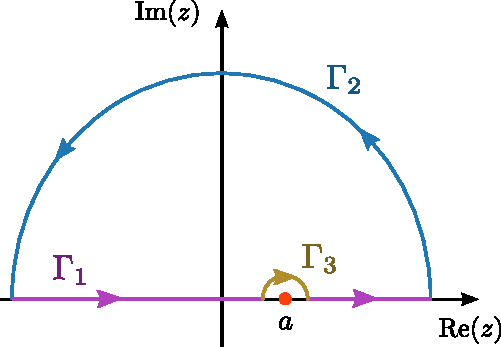
\includegraphics[width=0.5\textwidth]{principal_value_integral2}
\end{figure}

The solution procedure is very similar to the example worked out in
Section 8.4.3. From the properties of $f(z)$ given in the problem
statement, we can conclude that (i) the integrand is analytic on and
within the loop contour, so the residue theorem can be used; and (ii)
the integrand vanishes quickly enough far from the origin so that, by
Jordan's lemma, the integral over $\Gamma_2$ vanishes. Hence,
\begin{equation}
  I = i \pi f(a).
\end{equation}
 By relabelling the dummy variables
$x \rightarrow y$ and $a \rightarrow x$, we can write
\begin{equation}
  f(x) = -\frac{i}{\pi} \mathcal{P}\left[\int_{-\infty}^\infty \frac{f(y)}{y-x} dy \right].
\end{equation}
Let us now break up $f$ into its real and imaginary parts:
\begin{align}
  \mathrm{Re}[f(x)] + i \mathrm{Im}[f(x)]
  &= -\frac{i}{\pi} \mathcal{P}\left[\int_{-\infty}^\infty \frac{\mathrm{Re}[f(y)] + i \mathrm{Im}[f(y)]}{y-x} \;dy \right] \\
  &= \frac{1}{\pi} \mathcal{P}\left[\int_{-\infty}^\infty \frac{\mathrm{Im}[f(y)] -i\mathrm{Re}[f(y)]}{y-x} \;dy \right].
\end{align}
Equating the real and imaginary parts of the two sides, we obtain the
following two real equations, which are the Kramers-Kronig relations:
\begin{align}
  \mathrm{Re}[f(x)] &= \;\;\,\frac{1}{\pi} \mathcal{P}\left[\int_{-\infty}^\infty \frac{\mathrm{Im}[f(y)]}{y-x} \;dy \right] \\
  \mathrm{Im}[f(x)] &= -\frac{1}{\pi} \mathcal{P}\left[\int_{-\infty}^\infty \frac{\mathrm{Re}[f(y)]}{y-x} \; dy \right].
\end{align}

\end{enumerate}

\subsection*{9. Fourier Series and Fourier Transforms}

\begin{enumerate}
\item[3.]
The Fourier coefficients are given by
\begin{equation}
  f_n = \frac{1}{a} \int_{-a/2}^{\,a/2} dx\; e^{-i k_n x}\, f(x), \quad \mathrm{where}\;\, k_n = \frac{2\pi n}{a}.
\end{equation}
First, consider the case where $f(x)$ is real. Take the complex
conjugate of both sides:
\begin{align}
  f_n^* &= \frac{1}{a} \int_{-a/2}^{\,a/2} dx\; \left(e^{-i k_n x}\, f(x)\right)^* \\
  &= \frac{1}{a} \int_{-a/2}^{\,a/2} dx\; e^{i k_n x}\, f(x)^* \\
  &= \frac{1}{a} \int_{-a/2}^{\,a/2} dx\; e^{i k_n x}\, f(x) \\
  &= f_{-n}.
\end{align}
Hence,
\begin{equation}
  f_{n} = f_{-n}^*.
\end{equation}
For the second case, $f(x) = f(-x),$ perform a change of variables $x
= -u$ in the Fourier integral:
\begin{align}
  f_n &= \frac{1}{a} \int_{-a/2}^{\,a/2} du\; e^{i k_n u}\, f(u) \\
  &= f_{-n}.
\end{align}
For $f(x) = f(-x)^*$, the same change of variables gives
\begin{equation}
  f_n = f_n^*.
\end{equation}

\item[7.]
From the definition of the delta function as the narrow-peak limit of a
Gaussian wavepacket:
\begin{equation}
  \delta(ax) = \lim_{\gamma \rightarrow 0} \, \int_{-\infty}^\infty \frac{dk}{2\pi} \, e^{ikax} \, e^{-\gamma k^2}.
\end{equation}
Perform a change of variables $k = q/a$ and $\gamma = \gamma' \, a^2$:
\begin{align}
  \delta(ax) &= \lim_{\gamma' \rightarrow 0} \, \int_{-\infty}^\infty \frac{1}{a}\frac{dq}{2\pi} \, e^{iqx} \, e^{-\gamma' q^2} \\
  &= \frac{1}{a} \delta(x).
\end{align}

\item[8.]
Perform a change of variables from Cartesian coordinates $(x,y)$ to
polar coordinates $(r,\phi)$:
\begin{align}
   \int_{-\infty}^\infty dx \int_{-\infty}^\infty dy \; x^2\, \delta\left(\sqrt{x^2+y^2}-a\right) &= \int_0^{\infty} dr \int_{0}^{2\pi} rd\phi\, \cdot\, r^2\cos^2\phi\; \delta(r-a) \\
  &= \left(\int_0^{\infty} dr \, r^3\, \delta(r-a)\right) \left(\int_{0}^{2\pi}\!d\phi \, \cos^2\phi\right) \\
  &= \begin{cases}\pi a^3, & a \ge 0 \\ 0, & a < 0.\end{cases} 
\end{align}
\end{enumerate}

\subsection*{10. Green's Functions}

\begin{enumerate}
\item [2.]
For the over-damped oscillator, the Green's function is
\begin{equation}
  G(t,t') = \Theta(t-t')\, \frac{e^{-\gamma(t-t')}}{\Gamma} \sinh\big[\Gamma(t-t')\big], \quad\mathrm{where}\;\,\Gamma = \sqrt{\gamma^2 - \omega_0^2}.
\end{equation}
Hence, the response to the force $f$ is
\begin{equation}
  x(t) = \frac{1}{m\Gamma} \int^t_{-\infty} dt'\; e^{-\gamma(t-t')} \sinh\big[\Gamma(t-t')\big] f(t').
\end{equation}
From this, we get the following expression for the desired correlation
function:
\begin{multline}
  \langle x(t_1)\, x(t_2)\rangle = \frac{1}{m^2\Gamma^2} \int^{t_1}_{-\infty} dt' \int^{t_2}_{-\infty} dt'' \; e^{-\gamma(t_1-t')}\, e^{-\gamma(t_2-t'')} \\
  \times \sinh\big[\Gamma(t_1-t')\big] \sinh\big[\Gamma(t_2-t'')\big] \;
  \langle f(t') f(t'')\rangle.
\end{multline}
Note that the $\langle\cdots\rangle$ can be shifted inside the
integrals, because it represents taking the mean over independent sample
trajectories. Now, without loss of generality, let us take
\begin{equation}
  t_1 \ge t_2.
\end{equation}
Since $\langle f(t') f(t'')\rangle = A \delta(t'-t'')$ which vanishes
for $t' \ne t''$, the double integral only receives contributions from
values of $t'$ not exceeding $t_2$ (which is the upper limit of the
range for $t''$). Thus, we revise $\int^{t_1} dt'$ into $\int^{t_2}
dt'$. The delta function then reduces the double integral into a
single integral, which can be solved and simplified with a bit of
tedious algebra:
\begin{align}
  \langle x(t_1)\, x(t_2)\rangle &= \frac{A}{m^2\Gamma^2} e^{-\gamma(t_1+t_2)} \int^{t_2}_{-\infty} dt' e^{2\gamma t'} \sinh\big[\Gamma(t'-t_1)\big] \, \sinh\big[\Gamma(t'-t_2)\big] \\
  &= \frac{A}{8m^2\Gamma^2} e^{-\gamma(t_1+t_2)}\Bigg[\frac{e^{-\Gamma t_1} e^{(2\gamma+\Gamma)t_2}}{\gamma+\Gamma} + \frac{e^{\Gamma t_1}e^{(2\gamma-\Gamma)t_2}}{\gamma-\Gamma} \nonumber \\
    &\qquad\qquad\qquad\qquad\qquad - \frac{e^{-\Gamma t_1} e^{(\Gamma+2\gamma)t_2} + e^{\Gamma t_1} e^{(-\Gamma+2\gamma)t_2}}{\gamma}\Bigg] \\
  &= \frac{A}{8m^2\Gamma\gamma} \left[\frac{e^{-(\gamma-\Gamma)(t_1-t_2)}}{\gamma-\Gamma} - \frac{e^{-(\gamma+\Gamma)(t_1-t_2)}}{\gamma+\Gamma} \right].
\end{align}
Hence,
\begin{align}
  \left\langle [x(t+\Delta t) - x(t)]^2\right\rangle &= 2\Big[\left\langle x(t)^2\right\rangle - \left\langle x(t+\Delta t) x(t)\right\rangle\Big] \\
  &= \frac{A}{4m^2\Gamma\gamma} \left[\frac{1-e^{-(\gamma-\Gamma)\Delta t}}{\gamma-\Gamma} - \frac{1-e^{-(\gamma+\Gamma)\Delta t}}{\gamma+\Gamma} \right].
\end{align}
\end{enumerate}


\end{document}
